\documentclass{article}
\usepackage{amsmath}
\usepackage{textcomp}
\usepackage{xspace}
\usepackage{verbatim}
\usepackage{setspace}
\usepackage{cancel}
\usepackage{wrapfig}
\usepackage{graphicx}
\usepackage[fontsize=16pt]{fontsize}

\author{}
\date{}
\title{The Slash\\and £SD\\
\vspace{28pt}
\begin{normalsize}Applied Scholastics, Ferndale WA \end{normalsize}}

\begin{document}
\maketitle
\newpage

\section*{The '/' symbol}

The '/' symbol was used for many years in Europe and in the countries of the British Empire where currency was made up of Pounds, Shillings and Pence. It is called a solidus or a shilling mark and it is part of the Pounds, Shillings and Pence system - known as the the £sd system for short.\\

There were 12 pennies to a shilling and 20 shillings to a pound. The advantage of this £sd system over decimal, was that traders could divide a pound evenly into halves, thirds, quarters, fifths and sixths.\\

Financial accounts were commonly kept in Latin in the middle ages, so the names of the old Roman equivalents of coins were used in writing amounts of money instead of the actual names of the coins.\\

\newpage

\subsection*{Pounds}
The £ in £sd is a capital letter L from an old style of writing called Fraktur, which was a popular writing style that in Europe since the 1500s until the early 1900s. It stands for Libre Ponde, Latin for "weighed on scales," referring to a pound in weight of silver. The short stroke through the L is to indicate that it is an abbreviation.

\vspace{32pt}
\begin{center}
\includegraphics[width=\linewidth]{"fraktur cropped"}\\
\end{center}

This is Fraktur script. Note the shape of the capital letter 'L." 'Fraktur' means "broken." The letters of Fraktur script are made up of many short broken strokes.\\

\newpage

\subsection*{Shillings}
Shilling is an Old English word meaning $\frac{1}{20}^{th}$ of a pound.\\

The 'S' in £SD stands for 'solidus,' which was the name of a gold Roman coin. The solidus continued in use even after the fall of the Roman Empire until, after a shortage of gold in the eighth century, Pepin the Short, King of the Franks (the country that would become France), set up the new £sd system of currency with a new silver 'solidus' instead of gold. King Offa of Mercia, one of the kingdoms of Old England and which traded with the Franks, introduced the same system into England.\\

The 'S' for 'solidus' was used to refer to the shilling right up until the 1970s.\\

\subsection*{Pence}
D stood for 'denarius,' another Roman coin. In England, they replaced earlier silver pennies which were not part of the £sd system, but which continued to be called pennies. A penny was written as 1d.

\newpage

\subsection*{Long 'S'}

The long 's,' $\int$, is an old form of the letter 'S.'\\

Short 's'es were only for words ending in 's', before an apostrophe that indicated missing letters, before and after an 'f' (which looked too similar to a long 's'), and before the letters 'k' and 'b.'\\

The long 's' was used everywhere else. Double 's'es were written as a long 's' and a short 's.'\\

For example, 'success' was '$\int$ucce$\int$s,' 'satisfaction' was '$\int$atisfaction,' and 'ask' was 'a$\int$k.'\\

The long 's' fell out of use by the nineteenth century and it survives today, mainly, only in calculus where it stands for the Latin word 'summa' in certain equations.\\

\newpage

\section*{The Shilling mark}

\begin{wrapfigure}{r}{0.3\textwidth}
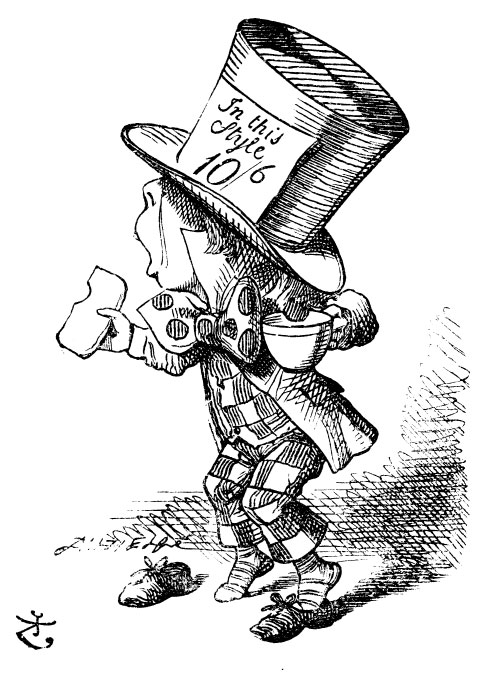
\includegraphics[width=0.6\textwidth]{madhatter}
\end{wrapfigure}

Amounts of Shillings were originally written with a long 's.' For example, 3 shillings and 6 pence was written as 3$\int$6d. The long 's' straightened out over the years until 3 shillings and 6 pence was written simply as 3/6d. This is the solidus symbol, also known as the slash or oblique symbol, that we have today.\\

The shilling mark appears in the Mad Hatter's hat in an illustration in the book Alice in Wonderland.\\

Whole numbers of shillings were written with a dash and a hyphen after the number. So, for example, one shilling was written as 1/-. Twelve shillings were written as 12/- or occasionally as 12s.

\begin{center}
\includegraphics[width=0.8\linewidth]{"DecimalConversionRates"}\\
\end{center}

A helpful chart from the UK in the 1970s when the old £sd system changed over to the new decimal system.\\
\
\newpage

\doublespacing

\begin{center}

Enquiries

\textbf{Applied Scholastics Ferndale}

Principal: Paula McLennan

mobile phone: 0431 683 306

email address: apsferndale@gmail.com

website: apsferndale.webs.com

\end{center}

\end{spacing}

\end{document}
